% !TeX spellcheck = da_DK
\subsection{Forstærker i opsamlingsblok}\label{Subsec:Forstaerker}
\subsubsection{Teori og design}
Til forstærkningen i opsamlingsblokken på \figref{kravblok} skal der benyttes en ikke-inverterende forstærker, da der ønskes, at inputtet og outputtet har samme polaritet. Ved en ikke-inverterende forstærker bliver inputtet tilkoblet direkte til den ikke-inverterende inputterminal, som har en impedans på $10^{12}\Omega$ indbygget i operationsforstærkeren\cite{Corporation1995}. Hvis der var en lav indgangsimpedans, hvilket der kan være i den inverterende terminal grundet designet, ville denne blok trække strøm fra inputsignalet, hvilket kan give  afvigelser i de efterfølgende blokke. \\
Kredsløbet består af en operationsforstærker kaldet TL$081$, som sidder i et closed-loop med modstandene R$1$ og R$2$, der udgør en spændingsdeler. Dette ses på \figref{fig:Forstaerker}.
\begin{figure}[H]
\centering
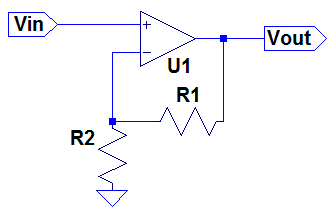
\includegraphics[scale=0.75]{figures/cProblemloesning/Forstaerker.PNG}
\caption{På figuren ses designet for en ikke-inverterende forstærker i en closed-loop konfiguration.}
\label{fig:Forstaerker}
\end{figure} 

\noindent Der er jævnfør afsnit \ref{OpsamlingsAfs} på side \pageref{OpsamlingsAfs} bestemt, at forstærkningen skal være en faktor $9.1$, hvilket svarer til $19.1808$dB. For at udregne R$1$ er R$2$ modstanden blevet valgt til $10$K$\Omega$. \cite{Nilsson2011} Ud fra dette er R$1$ blevet bestemt ved følgende udregning:
\begin{align}
9 = 1 + (\frac{R1}{10\text{K}\Omega})\\
R1 = 81\text{K}\Omega
\end{align}

\noindent R$1$ og R$2$ bliver brugt til at designe kredsløbet for en ikke-inverterende operationsforstærker. Dette kredsløb designes i LT-spice, som ses på \figref{fig:Forstaerker_faktor18}. 
\begin{figure}[H]
\centering
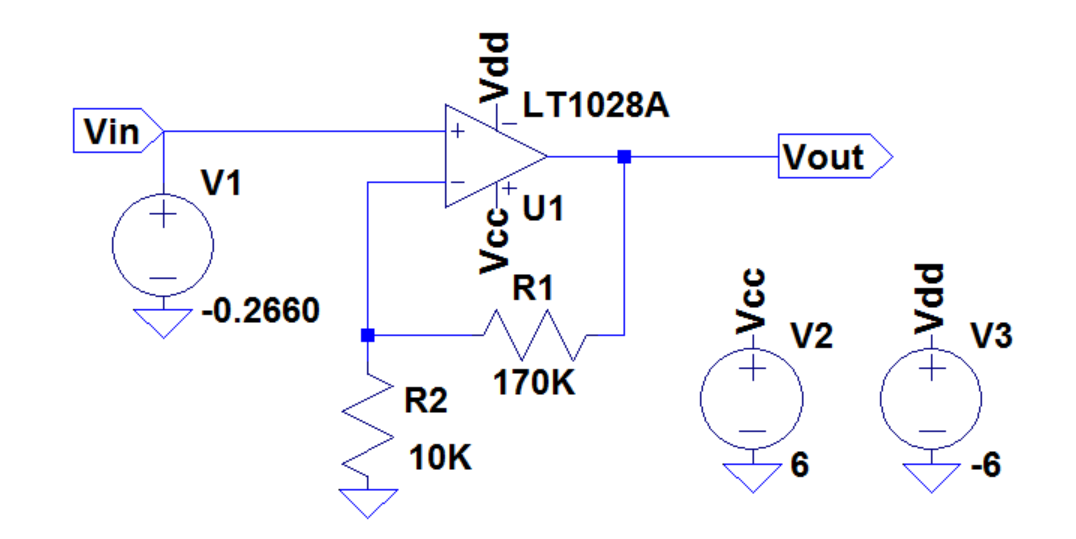
\includegraphics[scale=0.3]{figures/cProblemloesning/Forstaerker_faktor18.PNG}
\caption{På figuren ses designet at kredsløbet for en ikke-inverterende forstærker med to modstande. R$1$ og R$2$ har værdierne $81$K$\Omega$ og $10$K$\Omega$, hvilket giver en forstærkning med en faktor $9.1$.}
\label{fig:Forstaerker_faktor18}
\end{figure} 

\subsubsection{Simulering}\label{Subsec:Forstaerker_simu}
Der undersøges i to simuleringer, om forstærkeren virker ved det laveste input på $0.3233$V og højeste input på $0.3313$V, som er blevet udregnet igennem pilotforsøget. På \figref{fig:Forstaerker_faktor18_simulering} ses en simulering af dette.

\begin{figure}[H]
\centering
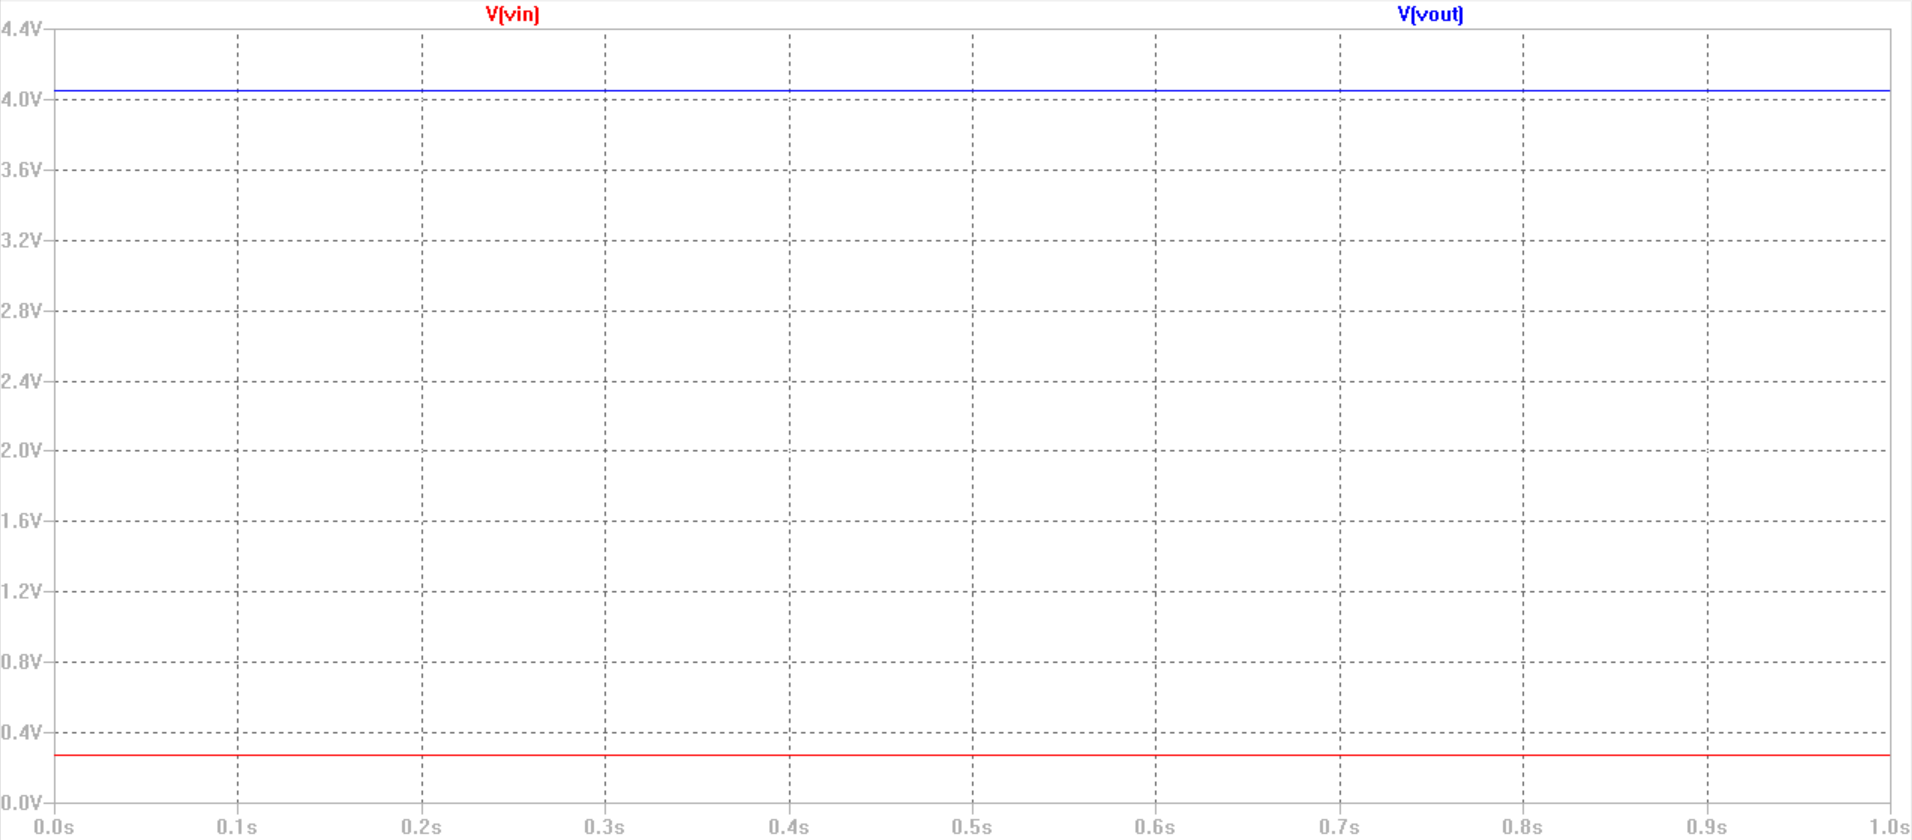
\includegraphics[scale=0.3]{figures/cProblemloesning/Forstaerker_faktor18_simulering.PNG}
\caption{På figuren ses en simulering af en ikke-inverterende forstærker, hvor der sker en forstærkning med en faktor $9.1$. Inputtet, $V_{in}$, er $0.3313$V, som bliver forstærket $9.1$ gange og derved giver ca. $3$V i outputtet, $V_{out}$.}
\label{fig:Forstaerker_faktor18_simulering}
\end{figure}

Der kan ses på \figref{fig:Forstaerker_faktor18_simulering}, at det forstærkede signal, kaldet $V_{out}$, er ca. $3$V, hvilket er ca. $9.1$ gange større end $V_{in}$, som i simuleringen er sat til $0.3313$V. Derved er der sket den ønskede forstærkning som forventet, da simuleringen er med ideelle komponenter. Derfor har de enkelte komponenter i denne simulering en lav tolerance, sammenlignet med komponenterne i et reelt kredsløb. \\
Resultaterne af de to simuleringer ses i \tableref{tab:forstarker18_sim}
\begin{table}[H]
	\centering
	\begin{tabular}{|l|l|l|l|l|}
		\hline
		\multicolumn{1}{|c|}{\textit{Inputsignalet}} & \multicolumn{1}{c|}{\textit{Forstærkning}} & \multicolumn{1}{c|}{Outputsignalet} &  \textit{Målte forstærkning}   & \textit{\begin{tabular}[c]{@{}l@{}}\% afvigelse\\ i forstærkning\end{tabular}} \\ \hline
		$0.3313$V      & $9.1$   & $3.0147$V    &  $9.10$  &   $0\%$  \\ \hline
%		$0$V           & 10       & $0$V          & $0.000206$V         & $0.0206$\%       \\ \hline
		-$0.3233$V     & $9.1$   & -$2.9417$V   &  $9.10$  &   $0\%$  \\ \hline
	\end{tabular}
	\caption{I tabellen ses resultaterne for simuleringerne med det laveste- og højeste input.}
	\label{tab:forstarker18_sim}
\end{table}
\noindent Der ses på afvigelserne, at der arbejdes med ideelle komponenter, da der er en lav afvigelse i outputtet ift. det forventede output. Derved fungerer kredsløbet teoretisk og kan implementeres.

\subsubsection{Implementering og test}
Ifølge det valgte design skal der benyttes to modstande på $10$K$\Omega$ og $81$K$\Omega$ til opbygningen af forstærkeren. Reelt findes der ikke en modstand på $81$K$\Omega$, hvorfor der istedet benyttes $82$K$\Omega$. Dette giver teoretisk en forskel på $1.235$\% i modstanden. Dette er det tætteste man kan komme på $81$K$\Omega$. Der kunne også benyttes en $150$K$\Omega$- og $180$K$\Omega$ modstand i parallel forbindelse, hvilket vil give $1.01$\% afvigelse. Disse komponenter vil også have afvigelser, hvorved den samlede procentvise afvigelse vil forøges. De to modstande blev målt inden testen, hvilket fremgår i \tableref{Tab:modstand_faktor18}.
\begin{table}[H]
	\centering
	\begin{tabular}{|l|l|l|}
		\hline
		\textit{Teoretisk} & \textit{Ved måling} & \textit{\% afvigelse} \\ \hline
		$10$K$\Omega$      & $10.0236$K$\Omega$    & $0.24$\%           \\ \hline
		$82$K$\Omega$      & $81.724$K$\Omega$     & $0.89$\%           \\ \hline
	\end{tabular}
	\caption{I tabellen ses det, at de to modstande afviger lidt fra deres teoretiske værdi, hvilket er forventet af reelle komponenter. Det er en acceptabel afvigelse ifølge tolerancerne i afsnit \ref{OpsamlingsAfs}, side \pageref{OpsamlingsAfs}. Modstandene kan derfor anvendes til implementeringen.}
	\label{Tab:modstand_faktor18}
\end{table}
\noindent Den $82$K$\Omega$ modstand har en $0.89\%$ afvigelse, men i dette tilfælde betragtes afvigelsen som positiv, da der ønskes en $81$K$\Omega$ modstand. Herefter blev kredsløbet implementeret. Til afbildning af signalet blev der benyttet et multimeter, som viste det forstærkede signal for de to spændingsniveauer. De aflæste resultater er angivet under "Output" i \tableref{Tab:faktor18_test}.\
\begin{table}[H]
	\centering
	\begin{tabular}{|l|l|l|l|l|}
		\hline
		\textit{Teoretisk input} & \textit{Målte input} & \textit{Output} & \% \textit{\begin{tabular}[c]{@{}l@{}}Faktiske\\ forstærkning\end{tabular}} & \textit{\begin{tabular}[c]{@{}l@{}}\% afvigelse\\ i forstærkning\end{tabular}} \\ \hline
		$0.3313$V   & $0.3310$V    & $3.0258$V       &    $9.14$   & $0.44\%$     \\ \hline
%		$0$V        & $0.3523$mV   & $3.5230$mV    & -$10$mV         & $38.49\%$      \\ \hline
		-$0.3233$V  & -$0.3231$V   & -$2.9612$V      &    $9.16$   & $0.66\%$     \\ \hline
	\end{tabular}
	\caption{I tabellen ses resultaterne fra testen med forstærkeren, der har en faktor $9.1$. Det maksimale og minimale input fra offsetjusteringen er blevet testet med.}
	\label{Tab:faktor18_test}
\end{table}
% Det "målte input" er her blevet målt med et multimeter. %For $0.3313$V er spændingen kommet direkte fra en strømforsyning, men for at undersøge forstærkningen af $-0.3233$V er det nødsaget at benytte offsettet, da spændingsforsyningen ikke kan levere en negativ spænding. Det var derfor forventet, at der kunne være en større afvigelse på målingerne med $-0.3233$V spænding, da denne spænding skulle igennem flere kredsløb. Inputtet i offsettet (som kan ses på \figref{fig:Offset_generisk}) var $1.3092$V og referencen var $1.6325$V. Derved skabes den negative spænding, som sendes videre til forstærkeren. Afvigelsen, som ville opstå grundet et ekstra kredsløb, ville være præsentabel for afvigelsen, som der også burde have været for de to andre signalers tests. Der ses i \tableref{Tab:faktor18_test}, at der ikke opstod større forstyrrelser, som gav ekstra afvigelse i det målte signal ift. det forventede signal. \\
Der ses ud fra testen, at forstærkeren overholder kravene fra afsnit \ref{OpsamlingsAfs}, side \pageref{OpsamlingsAfs}. Derudover ligger afvigelserne indenfor tolerancerne for forstærkningen, som er $\pm2\%$. Derfor anses disse afvigelser som acceptable.